\documentclass[11pt,a4paper]{article}

\usepackage[margin=2.5cm]{geometry}
\usepackage[T1]{fontenc}
\usepackage[utf8]{inputenc}
\usepackage{lmodern}
\usepackage{microtype}
\usepackage{amsmath,amssymb}
\usepackage{graphicx}
\usepackage{booktabs}
\usepackage{longtable}
\usepackage{array}
\usepackage{xcolor}
\usepackage{caption}
\usepackage{subcaption}
\usepackage{float}
\usepackage{hyperref}
\usepackage{enumitem}
\usepackage{fancyhdr}
\usepackage{lastpage}

\graphicspath{{figures/}}

\definecolor{linkblue}{RGB}{15,82,140}
\hypersetup{
  colorlinks=true,
  linkcolor=linkblue,
  citecolor=linkblue,
  urlcolor=linkblue,
  pdftitle={Photo Deblurring as an Inverse Problem},
  pdfauthor={Photo Deblurring IP Project}
}

\setlength{\parskip}{0.45em}
\setlength{\parindent}{0pt}
\setlist[itemize]{topsep=0.25em,itemsep=0.15em}
\setlist[enumerate]{topsep=0.25em,itemsep=0.15em}

\setlength{\headheight}{14pt}
\pagestyle{fancy}
\fancyhf{}
\lhead{Photo Deblurring IP Project}
\rhead{Final report}
\cfoot{\thepage\ of \pageref{LastPage}}

\newcommand{\figref}[1]{Figure~\ref{#1}}
\newcommand{\tabref}[1]{Table~\ref{#1}}
\newcommand{\eps}{\varepsilon}
\newcommand{\R}{\mathbb{R}}

\title{Photo Deblurring as an Inverse Problem\\\large Phase B project report}
\author{Gianni Gagliardi and Pietro Iaria\\Inverse Problems, Summer Semester 2026}
\date{\today}

\begin{document}
\maketitle

\begin{abstract}
This report summarizes a small photo deblurring project carried out in six steps. We generated blurred and noisy landscape images from clean RGB photographs, studied why the deblurring problem is ill-posed, implemented a standard Tikhonov baseline, built a sparse Matching Pursuit experiment, and compared these model-based approaches with DPIR, a recent plug-and-play method using a deep denoiser prior. The central model is
\[
  g = A f + \eps,
\]
where $f$ is the unknown clean image, $A$ is the motion-blur operator, $g$ is the observed degraded image, and $\eps$ is additive noise. The experiments show the expected behavior of an ill-posed inverse problem: blur suppresses frequencies, noise is easily amplified, and every reconstruction method must trade sharpness against stability. Qualitatively, DPIR gives the most natural reconstructions in the matched circular-convolution setting, but the comparison also shows that boundary assumptions and model mismatch matter.
\end{abstract}

\tableofcontents
\newpage

\section{Problem statement and notation}

The project task is photo deblurring. Starting from clean landscape images, we apply a known motion blur and additive noise, and then try to recover the original sharp image. Throughout the notebooks we use the notation
\begin{equation}
  g = A f + \eps.
  \label{eq:forward}
\end{equation}
Here $f \in [0,1]^{m \times n \times 3}$ is the clean RGB image, $A$ is the discrete blur operator, $g$ is the blurred/noisy observation, and $\eps$ denotes additive Gaussian noise. In vector form the same model is written as $\mathbf g = A \mathbf f + \boldsymbol\eps$.

The motion blur is horizontal with length $21$ pixels and angle $0^\circ$. Three noise levels were used: $\sigma_\eps = 0.02$, $0.05$, and $0.10$, measured on the normalized intensity scale $[0,1]$. The existing project observations were generated with reflective padding. This is important later, because some deblurring formulas, especially FFT-based ones, naturally assume circular convolution instead.

\section{Step 1: data preparation and forward model}

The raw landscape photographs were converted to RGB, center-cropped, and resized to a common resolution of $512 \times 512$. This keeps the experiment simple: all images have the same shape and the same blur/noise settings. The prepared clean images and their blurred/noisy observations are shown in \figref{fig:data-overview}.

\begin{figure}[H]
  \centering
  \includegraphics[width=\textwidth]{step6_data_overview.png}
  \caption{Clean images $f$ and existing blurred/noisy observations $g$ for the three noise levels. The observations were generated with reflective padding.}
  \label{fig:data-overview}
\end{figure}

The discrete point-spread function (PSF) is normalized so that image brightness is preserved before clipping. In code, the same kernel is reused across the standard, sparse, and recent-method experiments whenever possible. The main difference between experiments is not the kernel itself, but the assumed boundary condition and the chosen prior or regularization.

\section{Step 2: ill-posedness analysis}

Deblurring is unstable because the blur operator removes or strongly attenuates information. In the Fourier domain, a horizontal motion blur has a response with small values near certain frequencies. If we tried to invert $A$ naively, these small values would appear in the denominator, so even small noise in $g$ would be amplified.

The notebook also constructs a small explicit blur matrix as an illustrative finite-dimensional model. The singular values decay strongly, which is another view of the same problem: some directions in image space are almost invisible after applying the blur. \figref{fig:illposedness} condenses this part of the analysis.

\begin{figure}[H]
  \centering
  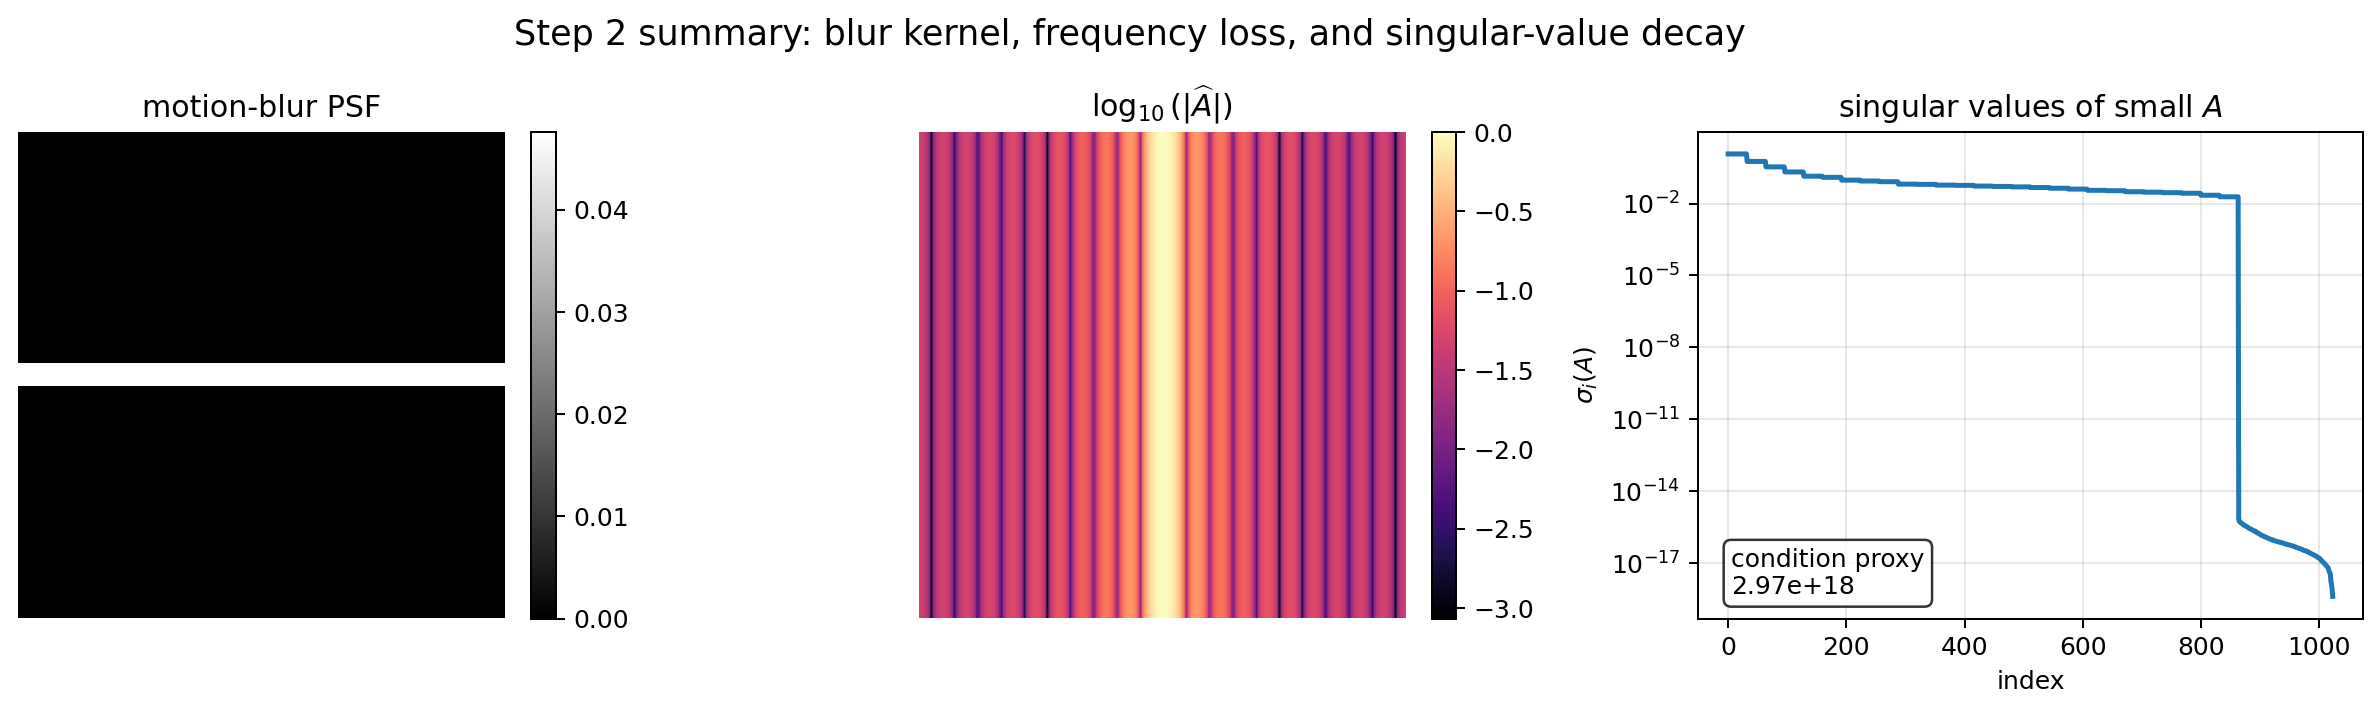
\includegraphics[width=0.95\textwidth]{step6_step2_illposedness_summary.png}
  \caption{Step 2 summary. Left: the horizontal motion-blur PSF. Middle: logarithmic Fourier magnitude of the blur response. Right: singular-value decay of a small representative blur matrix. The small Fourier values and small singular values explain why inverse filtering is noise-sensitive.}
  \label{fig:illposedness}
\end{figure}

A useful mental picture is this: the observation $g$ is not just a less sharp version of $f$. Some high-frequency information has been mixed and weakened by $A$. Regularization is therefore not an optional cosmetic step; it is needed to define a stable reconstruction.

\section{Step 3: standard method - Tikhonov regularization}

As a standard model-based baseline, we used zero-order Tikhonov regularization \cite{tikhonov1977solutions}. The reconstruction is defined by
\begin{equation}
  f_\lambda
  = \arg\min_f
  \left\{ \|Af-g\|_2^2 + \lambda \|f\|_2^2 \right\}.
  \label{eq:tikhonov}
\end{equation}
The first term enforces agreement with the observation, while the second term penalizes large solution norms. The parameter $\lambda > 0$ controls the trade-off. A small $\lambda$ tries to invert the blur more aggressively but can amplify noise; a large $\lambda$ is more stable but oversmooths the image.

Because the blur is horizontal, the Step 3 notebook builds a one-dimensional reflective blur matrix $B$ for each row. For each RGB channel, the forward model can be written row-wise as
\begin{equation}
  g_{r,c} = B f_{r,c} + \eps_{r,c},
\end{equation}
where $r$ is the row index and $c$ is the color channel. The reconstruction is computed efficiently from the singular value decomposition of $B$. The notebook uses an L-curve to select a representative $\lambda$, balancing the residual norm $\rho = \|Af-g\|_2$ and solution norm $\eta = \|f\|_2$.

\begin{figure}[H]
  \centering
  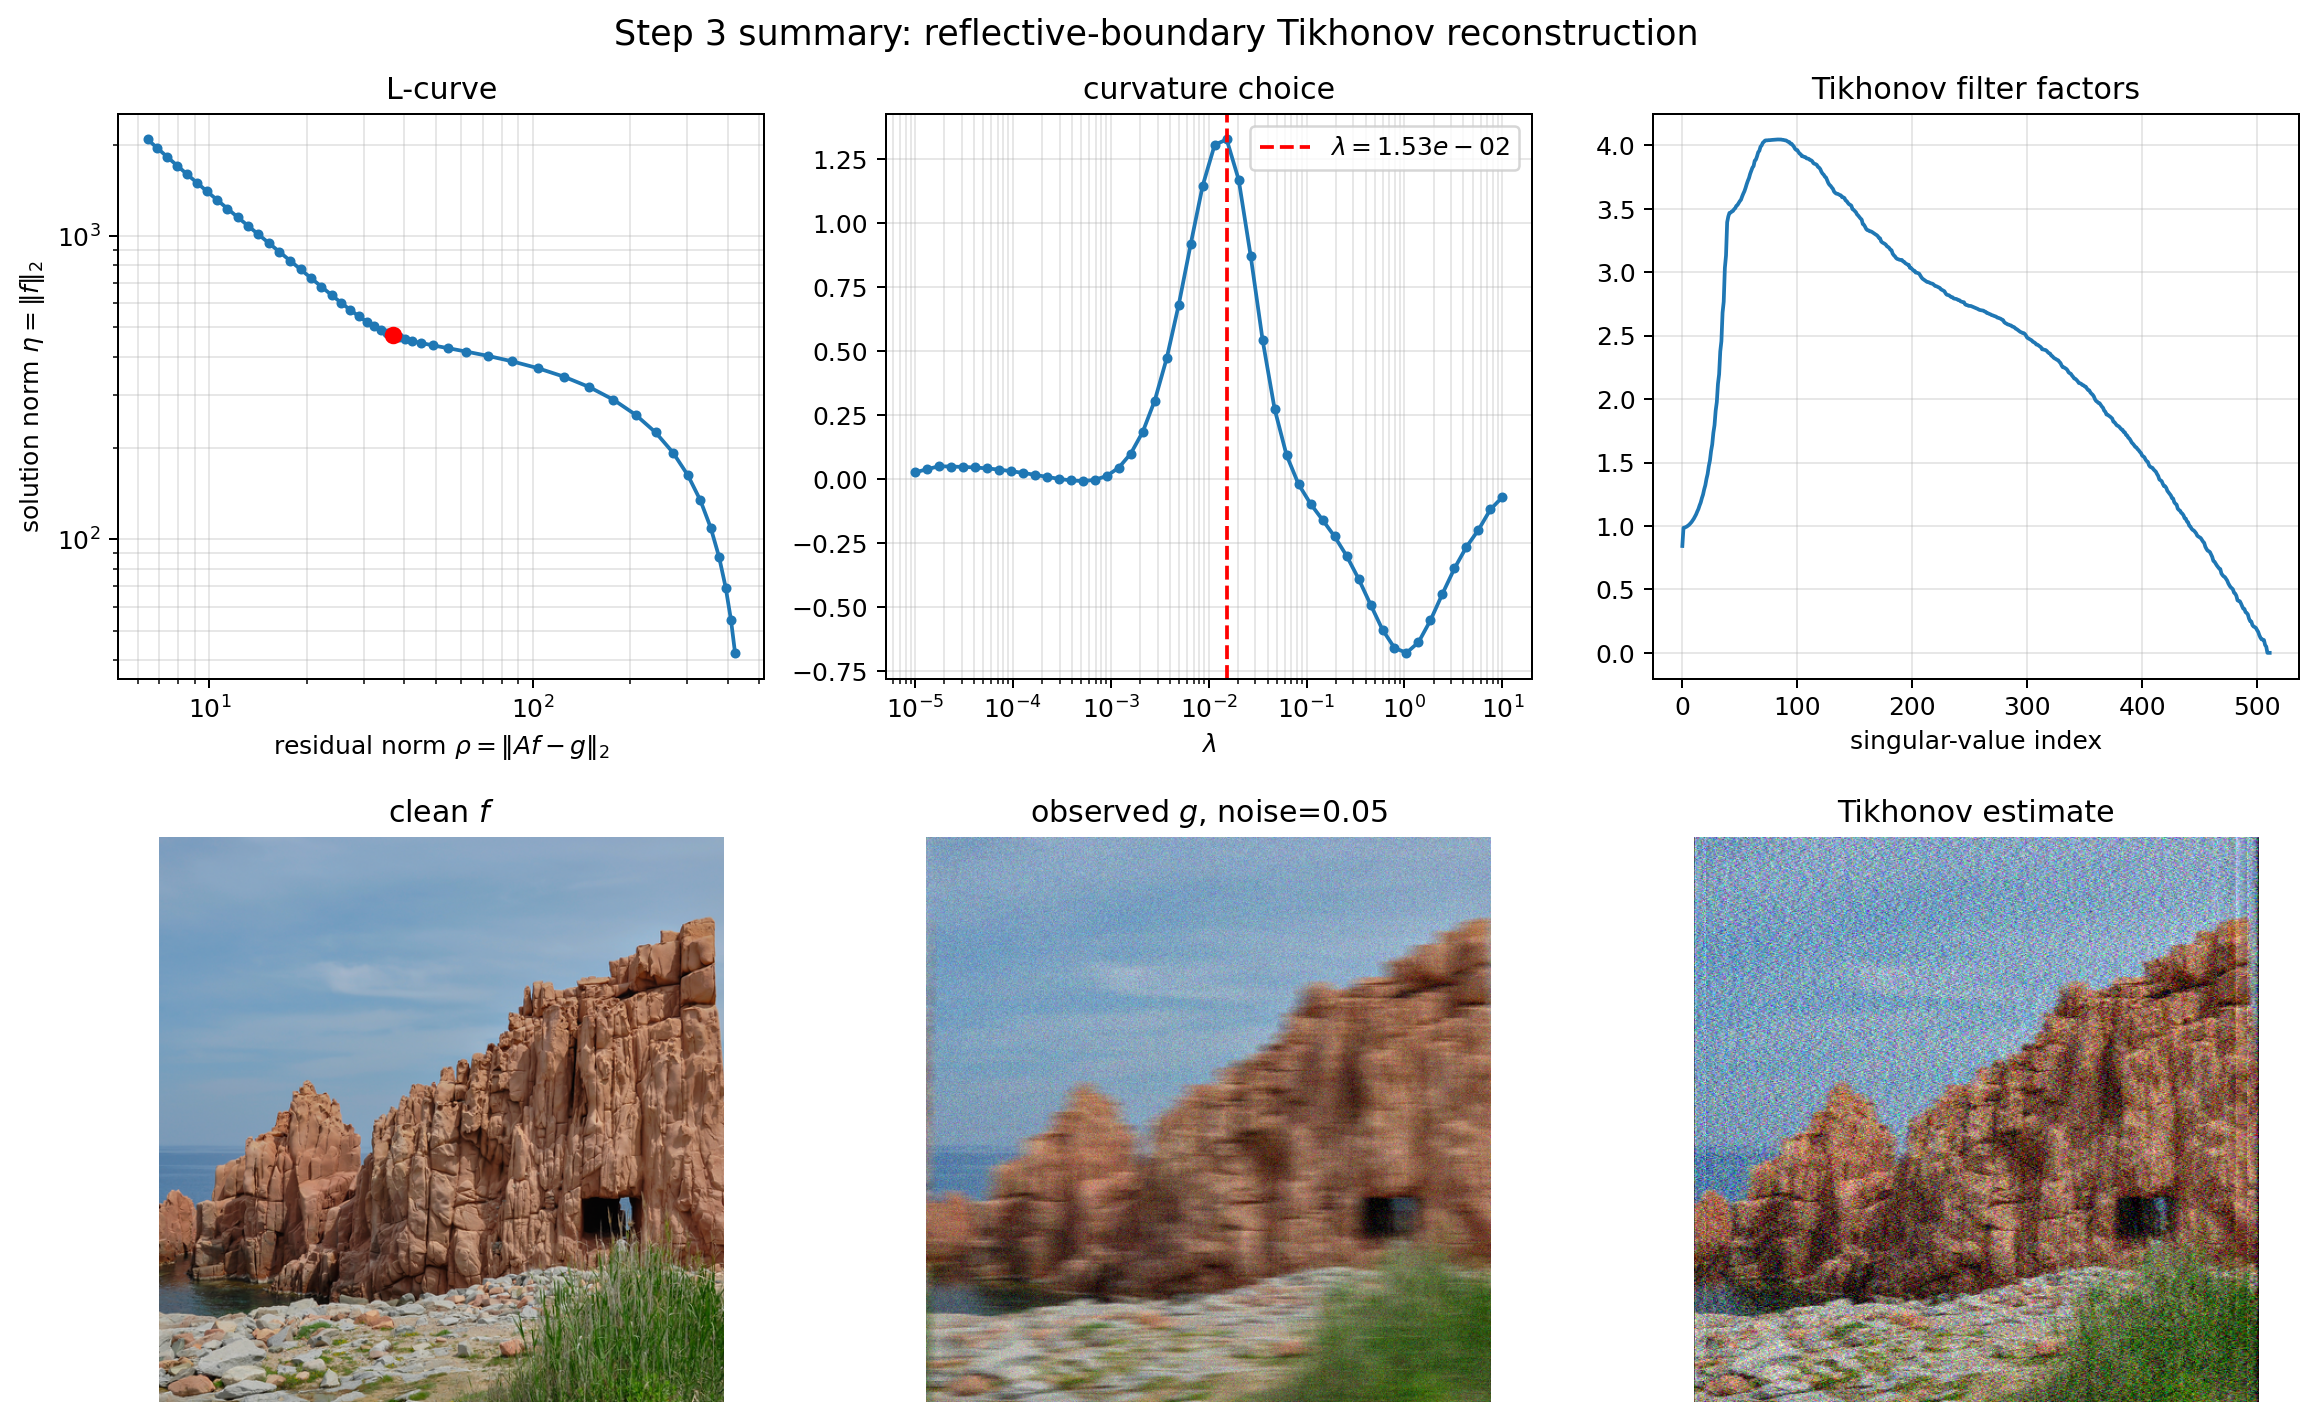
\includegraphics[width=0.95\textwidth]{step6_step3_tikhonov_representative.png}
  \caption{Step 3 Tikhonov summary for one representative image/noise setting. The top row shows the L-curve, curvature-based parameter choice, and filter factors. The bottom row shows the clean image, observation, and Tikhonov estimate.}
  \label{fig:tikhonov}
\end{figure}

The Tikhonov result is useful because it is transparent and closely tied to the forward model. At the same time, it has a very simple prior: it mainly controls energy, not edges or natural-image structure. This is why the output can remain blurry or show artifacts when the chosen $\lambda$ is not ideal for all image features.

\section{Step 4: sparse Matching Pursuit method}

For the sparse method, we followed the notation from the exercise sheet and used a Haar-wavelet representation. In simplified form, the image is written as
\begin{equation}
  f \approx \Psi s,
\end{equation}
where $\Psi$ is a Haar basis and $s$ is expected to be sparse or at least compressible. Combining this with the forward model gives
\begin{equation}
  g' = A \Psi s + \eps = \Phi s + \eps.
\end{equation}
Matching Pursuit greedily selects atoms that best explain the current residual \cite{mallat1993matching}. Rather than solving for all coefficients at once, it repeatedly finds a promising coefficient, updates the approximation, and reduces the residual.

In practice, full RGB Matching Pursuit at $512 \times 512$ is too expensive for an interactive notebook. We therefore used full-size grayscale images and the row-wise horizontal operator $A_2$ as the main sparse experiment. The observations for this step were generated in a matched way, using the same operator as the reconstruction. This choice avoids blaming Matching Pursuit for artifacts that would actually come from an operator mismatch.

\begin{figure}[H]
  \centering
  \includegraphics[width=\textwidth,height=0.82\textheight,keepaspectratio]{step6_sparse_mp_grayscale_overview.png}
  \caption{Step 4 sparse Matching Pursuit results for full-size grayscale images. The method captures broad structures, but the reconstructions are visibly blocky and lose fine detail because the simple Haar dictionary and limited number of selected atoms are not rich enough for high-quality natural-image deblurring.}
  \label{fig:sparse}
\end{figure}

The sparse method is valuable as a learning experiment. It makes the idea of a prior very concrete: we explicitly ask for a representation using few wavelet atoms. But visually it is not competitive with the stronger DPIR prior used later, especially for natural color photographs.

\section{Step 5: recent method - DPIR}

The recent method is DPIR, ``Plug-and-Play Image Restoration with Deep Denoiser Prior'' \cite{zhang2022dpir}. We used the official PyTorch implementation as a local ignored dependency \cite{dpirgithub}. DPIR is not just a neural network applied once to the blurry image. It is an iterative plug-and-play method: the known degradation model $A$ still appears in a data-consistency step, while a pretrained DRUNet denoiser acts as an implicit natural-image prior.

A helpful way to understand the method is through a half-quadratic splitting viewpoint. One alternates between
\begin{itemize}
  \item a data step, which pulls the current image toward agreement with $g = Af + \eps$;
  \item a denoising step, which applies the learned denoiser and pulls the image toward the set of natural-looking images.
\end{itemize}
The DPIR schedule uses parameters such as $\rho$ and the denoiser noise level $\sigma$. Informally, $\rho$ controls how strongly the splitting variable is tied to the data-consistency update, while the denoiser $\sigma$ controls how aggressively DRUNet removes noise and artifacts. Larger denoiser strength stabilizes the reconstruction but can remove fine texture.

\subsection{Boundary-condition mismatch}

The existing project images use reflective padding. DPIR's FFT deblurring update assumes circular convolution. Therefore, applying DPIR to the existing observations is a model-mismatch experiment: the observation $g$ was created with one operator, while DPIR uses a slightly different $A$ during reconstruction. This is not a minor technicality. Boundary conditions can change the behavior near image edges and can also influence ringing or residual blur.

To separate this issue from the method itself, the Step 5 notebook also generates controlled observations with circular convolution. These matched examples use the same boundary model that DPIR assumes.

\begin{figure}[H]
  \centering
  \includegraphics[width=\textwidth,height=0.82\textheight,keepaspectratio]{step6_dpir_existing_mismatch_overview.png}
  \caption{DPIR on the existing project observations. These are reflective-padding/circular-convolution mismatch cases. The results are useful, but boundary-related artifacts should not be interpreted as only a failure of the denoiser.}
  \label{fig:dpir-mismatch}
\end{figure}

\begin{figure}[H]
  \centering
  \includegraphics[width=\textwidth,height=0.82\textheight,keepaspectratio]{step6_dpir_circular_matched_overview.png}
  \caption{DPIR on controlled circular-convolution observations. Here the degradation model used to create $g$ matches DPIR's FFT/circular model, so this is the cleaner test of DPIR's intended setting.}
  \label{fig:dpir-matched}
\end{figure}

Qualitatively, DPIR gives the most natural results in this project. The matched circular-convolution results show strong denoising and partial deblurring while preserving large image structures. As the noise level increases, the outputs become smoother. This is expected: the method must rely more heavily on the prior when the data are less trustworthy.

\section{Step 6: final qualitative comparison}

The final notebook collects the figures needed for the report. We intentionally did not add a numerical PSNR/SSIM table at this stage, because the final task here was to prepare a concise visual report. The representative comparison in \figref{fig:comparison} summarizes the main observations.

\begin{figure}[H]
  \centering
  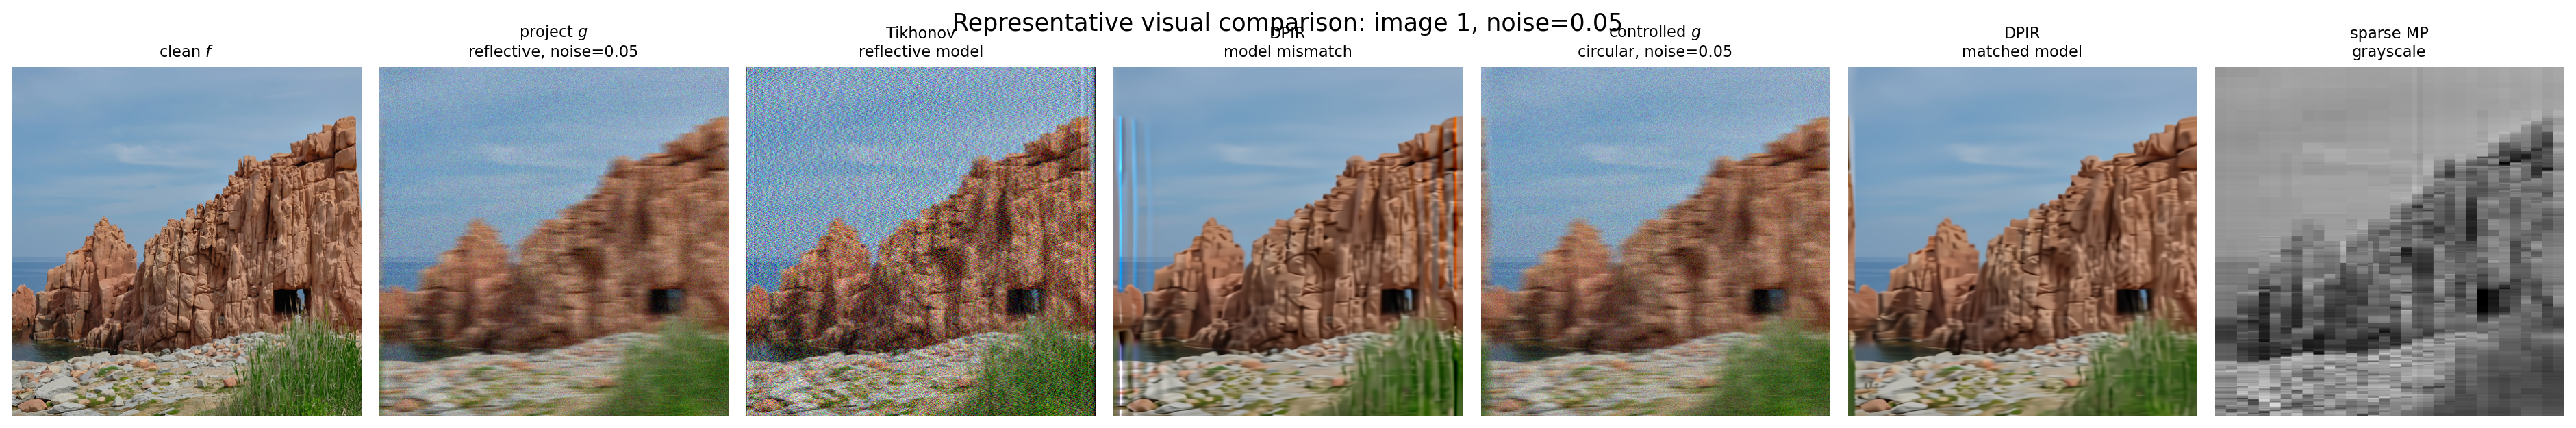
\includegraphics[width=\textwidth]{step6_representative_comparison_image1_sigma005.png}
  \caption{Representative visual comparison for image 1 at noise level $0.05$. The figure includes the clean image, the reflective-padding observation, Tikhonov, DPIR under model mismatch, the controlled circular observation, matched DPIR, and sparse Matching Pursuit in grayscale.}
  \label{fig:comparison}
\end{figure}

The main qualitative conclusions are:
\begin{itemize}
  \item Step 2 confirms that the inverse problem is genuinely ill-posed: blur attenuates information and small singular values make direct inversion unstable.
  \item Tikhonov regularization is mathematically clean and reproducible, but its simple prior cannot fully recover natural-image detail.
  \item Sparse Matching Pursuit clearly demonstrates the sparse-prior idea, but the simple Haar setup is too limited for visually convincing full-size deblurring.
  \item DPIR is visually strongest, especially when the forward model is matched. It removes noise well and produces natural-looking images, but can oversmooth fine textures and depends on pretrained weights.
  \item Boundary assumptions matter. The difference between reflective and circular convolution is a real model-mismatch limitation, not just an implementation detail.
\end{itemize}

\section{Discussion}

The project started from a classical inverse-problem viewpoint and gradually added stronger priors. This progression is useful because it shows what each ingredient contributes. The forward model $A$ matters in every method. If $A$ is wrong, even a strong prior can produce misleading results. The prior also matters: Tikhonov uses a very simple energy penalty, Matching Pursuit uses explicit sparsity in a Haar basis, and DPIR uses a learned natural-image denoiser.

In terms of visual quality, the modern learned prior clearly helps. DPIR is much better at producing natural-looking images than the sparse Haar Matching Pursuit baseline, and it is less limited than zero-order Tikhonov. Still, this should not be read as ``deep learning solves the inverse problem''. DPIR works well here because it combines a data-consistency step with a strong denoiser prior. It also requires more setup, external weights, and a careful statement of the boundary model.

The most important limitation of the current comparison is that it is qualitative. A fuller evaluation would add a consistent metric table, runtime measurements, and parameter sweeps for all methods. Another limitation is that the sparse method was reduced to grayscale for computational reasons. That was a practical decision, but it means the sparse result is not a full RGB competitor to DPIR.

\section{Reproducibility}

The repository contains the complete notebooks and scripts used for the project. The project repository is available at \href{https://github.com/gianni-1/Photodeblurring_IPProject}{\texttt{github.com/gianni-1/Photodeblurring\_IPProject}}.

\begin{itemize}
  \item Step 1: image preparation and degradation generation in the preprocessing script and exploratory notebook.
  \item Step 2: ill-posedness analysis in \texttt{src/step2.ipynb}.
  \item Step 3: Tikhonov deconvolution in \texttt{src/photodeblur/step3 copy.ipynb}.
  \item Step 4: sparse Matching Pursuit in \texttt{src/step4\_sparse\_matching\_pursuit.ipynb}.
  \item Step 5: DPIR feasibility and final notebooks in \texttt{src/step5\_dpir\_feasibility.ipynb} and \texttt{src/step5\_dpir\_final.ipynb}.
  \item Step 6: final figure collection in \texttt{src/step6\_final\_figures.ipynb}.
\end{itemize}
Large external dependencies, especially the DPIR repository and pretrained weights, are intentionally kept outside version control under \texttt{external/}.

\appendix

\bibliographystyle{plain}
\bibliography{references}

\end{document}
